\chapter{Validierung} \label{Validierung}

%%%%%%%%%%%%%%%%%%%%%%%%%%%%%%%%%%%%%%%%%%%%%%%%%%%%%%%%%%%%%%%%
% Überblick
%%%%%%%%%%%%%%%%%%%%%%%%%%%%%%%%%%%%%%%%%%%%%%%%%%%%%%%%%%%%%%%%
\section{Überblick} \label{ValidUeberblick}
Ziel der Validierungsphase ist das Testen auf dem fertigen Board, anhand von Testpersonen. Der Weg bis dahin muss aber ebenfalls kontrolliert und geprüft sein. Zur Sicherstellung der Funktionalität werden die Komponenten einzeln als auch gesamthaft getestet. 
Jeder Hardware-Bestandteil – Brett, Steuerung, Stromversorgung und Motoransteuerung - hat also sein eigenes Testkonzept.

%%%%%%%%%%%%%%%%%%%%%%%%%%%%%%%%%%%%%%%%%%%%%%%%%%%%%%%%%%%%%%%%
% Brett
%%%%%%%%%%%%%%%%%%%%%%%%%%%%%%%%%%%%%%%%%%%%%%%%%%%%%%%%%%%%%%%%
\section{Brett} \label{ValidBrett}
Das Brett selber, die gepressten Birkenholzplatten, dessen Bearbeitung und die darauf befindliche Stromleiter und Gehäuse wurden einem Stabilitätstest unterzogen, wo geprüft wurde, ob die Komponenten ein Ausreizen der Flexibilität des Brettes vertragen. Die Verbindungen wurden durchgemessen. Es wurde keine Widerstandserhöhung festgestellt. Das Brett selber ist auch nicht zerbrochen.

%%%%%%%%%%%%%%%%%%%%%%%%%%%%%%%%%%%%%%%%%%%%%%%%%%%%%%%%%%%%%%%%
% Magic Glove
%%%%%%%%%%%%%%%%%%%%%%%%%%%%%%%%%%%%%%%%%%%%%%%%%%%%%%%%%%%%%%%%
\section{Steuerung - Magic Glove} \label{ValidSteuerMagicGlove}
Für die Validierung des Magic Glove wurde eine Hand 3d-gedruckt und ein seperater Empfänger mit einem Arduino gebaut, welcher die empfangenen Daten über eine serielle Verbindung an einen Computer sendet. Die Hand wird nun von Minima zu Maxima gebeugt und die gemessenen Werte aufgezeichnet. Somit kann garantiert werden, dass der maximale Bewegungsradius aufgelöst wird und die Daten korrekt gesendet werden.
\begin{figure} [H]
	\centering
	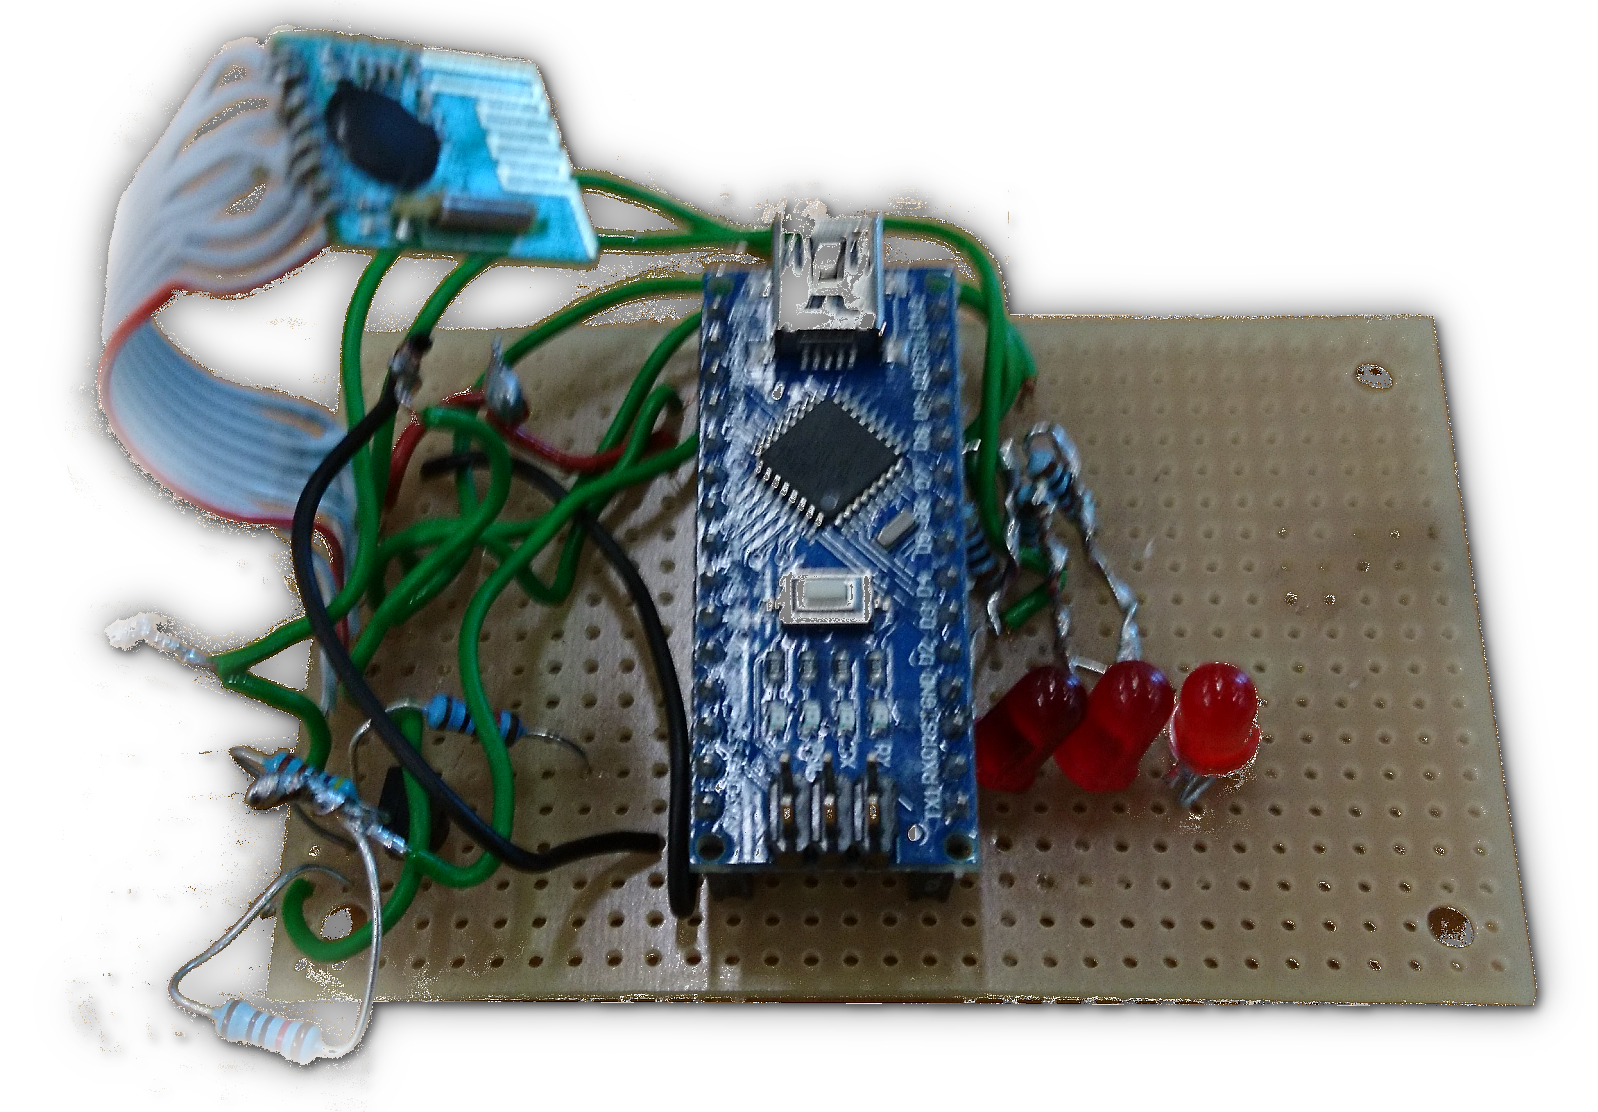
\includegraphics[scale=0.2]{images/receiver}
	\caption{Empfänger zur Validierung des Magic Glove}
	\label{fig:statediagrammbatterie}
\end{figure}
%%%%%%%%%%%%%%%%%%%%%%%%%%%%%%%%%%%%%%%%%%%%%%%%%%%%%%%%%%%%%%%%
% Stromversorgung
%%%%%%%%%%%%%%%%%%%%%%%%%%%%%%%%%%%%%%%%%%%%%%%%%%%%%%%%%%%%%%%%
\section{Stromversorgung} \label{ValidStromversorgung}

%%%%%%%%%%%%%%%%%%%%%%%%%%%%%%%%%%%%%%%%%%%%%%%%%%%%%%%%%%%%%%%%
% MC
Damit die Ergebnisse reproduzierbar sind, wird die Stromversorgung auf einem Prüfstand getestet. In der ersten Validierungsphase wird der Print und die Software ohne Akku getestet, welcher dann in der zweiten Valierungsphase angeschlossen wird. \textbf{Achtung:} Da es sich beim Akku um einen Lithium-Polymer Akku handelt, welcher einen Spitzenstrom von bis zu 500A liefert, sollte der Print zuerst auf allfälligen Kurzschluss geprüft werden.   

\textbf{Hardware}
\begin{itemize}
	\item Funktion der FETs
	\item Messung der Spannungen
	\item Ausmessung des Highside-Driver
\end{itemize}
\textbf{Software}
\begin{itemize}
	\item Einlesen Spannung und Ströme
	\item PWM-Regelung
	\item Balancing Steuerung
\end{itemize}

\subsection*{Hardware}
\subsubsection*{FETs}
Als erstes werde die FETs des Balancing der Reihe nach eingeschaltet. Dabei wird jeweils eine Spannung von 4.2V zwischen Zellanschluss 6 und 5, Zellanschluss 5 und 4 usw. angeschlossen. Sobald die richtige Spannung angeschlossen ist und derjenige FET durchgeschaltet ist, sollte einen Strom von 100mA fliessen.

Weiter werden die FETs getestet, welche die Spannung zum Motorkontrollboard steuern. Dabei wird einen Leistungswiderstand auf Masse geschaltet. 
\begin{center}
	\begin{tabular}{|c|c|}
		\hline 
		Versorgungsspannung & $25V$ \\ \hline
		Lastwiderstand & $2.5\Omega$ \\ \hline
	\end{tabular} 
	\captionof{table}{Messbedingungen FETs zu Motorcontroll}
	\label{tab:fetmessbedzumotorcontrol}
\end{center}

Nun sollte ein Strom von rund 10A fliessen. Dabei sollten die FETs nur leicht oder gar nicht warm werden. Der FET welcher fürs Laden zuständig ist, wird bei der Ausmessung des Highside-Driver getestet.

\subsubsection*{Spannungsmessung}
Nun werden die einzelnen Spannungsteiler ausgemessen. Dabei wird am Balancing Anschluss die einzelnen Zellen angeschlossen. Weiter wird die Ladespannung angeschlossen. Nun sollte an den Spannungsteiler gemessen werden. Der Akku sollte voll geladen sein und die Spannungsteiler dürfen die Microcontrollerspeissung nicht überschreiten.

\begin{center}
	\begin{tabular}{|c|c|}
		\hline 
		Versorgungsspannung Batterieseitig & $25V$ \\ \hline
		Versorgungsspannung Ladeseitig & $30V$ \\ \hline
		Versorgungsspannung Mikrokontroller & $5V$ \\ \hline
		Versorgungsspannung Highside-Driver & $15V$ \\ \hline
		Alle sechs Balancing Spannungsteiler & $4.2V$ \\ \hline
		Spannungsteiler Ladeseitig & $2.1V$ \\ \hline
		
	\end{tabular} 
	\captionof{table}{Spannungsmessungen}
	\label{tab:Spannungsmessungen}
\end{center}

\subsubsection*{Highside-Driver}
\label{Highside-Driver}
Damit der Highside-Driver getestet werden kann, sollte die Batterie entfernt und einen Leistungswiderstand von rund 5$\omega$ angeschlossen werden. Der Highside-Driver wird dabei extern mit 15V gespiessen. Als erstes wird am Mikrocontroller einen PWM mit 50\% Duty-Cycle ausgegeben. Dabei sollte am Ausgang des Highside-Driver dasselbe Signal mit 15V Spannungsspitze anliegen. Nun wird eine externe Ladespannung angeschlossen. Diese liegt für Testzwecke bei 15V. Dabei sollte die Strombegrenzung auf 3A eingestellt sein. Nun wird der Duty-Cycle ständig erhöht. Dabei wird der Strom beim Leistungswiderstand gemessen und mit nachfolgender Tabelle abgeglichen.

\begin{center}
	\begin{tabular}{|c|c|}
		\hline 
		Duty-Cycle: 0\% & $0A$ \\ \hline
		Duty-Cycle: 20\% & $0.6A$ \\ \hline
		Duty-Cycle: 40\% & $1.2A$ \\ \hline
		Duty-Cycle: 60\% & $1.8A$ \\ \hline
		Duty-Cycle: 80\% & $2.4A$ \\ \hline
	\end{tabular} 
	\captionof{table}{Ladestrom bei verschiedenen Duty-Cycle}
	\label{tab:LadestromHighsideDriver}
\end{center}

Einen Duty-Cycle von 100\% wird nicht geprüft, da der Highside-Driver nicht dazu ausgelegt ist einen FET dauerhaft durch zusteuern.

\subsection*{Software}
Um diese Ergebnisse zu überprüfen, muss am USART des Mikrocontroller ein TTL-Kabel angeschlossen werden.

\subsubsection*{ADC}
Um die einzelnen Zellen auszulesen, kann die Batterie sowie eine Ladespannung von mindestens 30V angeschlossen werden. Dabei werden die einzelnen Spannungen jede Sekunde einmal über den USART Port ausgegeben. Dabei sollte die Spannung mit dem Fluke gemessen und überprüft werden. Um denn Strom zu messen, wird die Messung gleich wie in Kapitel \ref{Highside-Driver} aufgebaut. 

\subsubsection*{PWM-Regelung}
Um zu überprüfen wird Software-Seitig ein vordefinierter Strom eingestellt. Dabei wird anstatt der Akku ein veränderbarer Leistungswiderstand am Ausgang angeschlossen. Nun wird der Widerstand verändert und überprüft, ob die Software richtig nachregelt.
\begin{center}
	\begin{tabular}{|c|c|}
		\hline 
		Teststrom & $1A$ \\ \hline
		${f}_{PWM}$ & $32kH$ \\ \hline
	\end{tabular} 
	\captionof{table}{Ladestrom bei verschiedenen Duty-Cycle}
	\label{tab:LadestromHighsideDriver}
\end{center}
\todo{Wenn möglich, sollte hier noch ein Bild eingefügt werden} 

\subsubsection{Balancing-Regelung}
Für diese Validierung wird jeweils eine Spannung an den Zellen Anschlüssen angeschlossen. Dabei wird überprüft, ob die Software bei den jeweiligen Zellen die FETs durch steuert, um  die gleiche Spannung wie bei den anderen Zellen zu erreichen.


%\begin{itemize}
%\item Einlesen Spannung und Ströme
%\item PWM-Regelung
%\item Balancing Steuerung
%\end{itemize}

%%%%%%%%%%%%%%%%%%%%%%%%%%%%%%%%%%%%%%%%%%%%%%%%%%%%%%%%%%%%%%%%
\section{Motoransteuerung} \label{ValidMotoransteuerung}
Um reproduzierbare Ergebnisse zu erzielen, wird die Motoransteuerung auf einem Prüfstand getestet. Der Motor wird ohne Last befestigt und die Schaltung von einem Netzteil gespiesen. Weiter wird die Motoransteuerung in einzelnen Blöcken validiert. Dabei wird unterschieden in Hardware und Software.\\
\\
\textbf{Hardware}
\begin{itemize}
	\item Funktion der FETs
	\item Spannungsmessung mit Spannungsteiler
\end{itemize}
\textbf{Software}
\begin{itemize}
	\item Einlesen der Spannungen und Ströme
	\item SVPWM Raumvektormodulation
	\item Positions- und Geschwindigkeitsbeobachter
	\item D und Q Stromregler
\end{itemize}

\subsection*{Hardware}
\subsubsection*{FETs}
Die FETs werden der Reihe nach von der Software eingeschalten. Zum Test der High-Side FETs wird am Ausgang ein Widerstand auf Masse geschaltet. So kann die Spannung am Ausgang gemessen und aufgezeichnet werden. Zusätzlich wird die Gatespannung gemessen.

\begin{center}
	\begin{tabular}{|c|c|}
		\hline 
		Versorgungsspannung & $15V$ \\ \hline
		Lastwiderstand & $1k\Omega$ \\ \hline
		Gatestrom Treiber & $1.7A$ \\ \hline
	\end{tabular} 
	\captionof{table}{Messbedingungen FETs}
	\label{tab:fetmessbed}
\end{center}

Zur Gunsten der Übersichtlichkeit wird nur die Messung eines FETs dargestellt.

\begin{figure} [H]
	\centering
	
\includegraphics[width=0.5\linewidth]{images/placeholder.png}
	\caption{Einschalten High-Side FET}
	\label{fig:hsfet}
\end{figure}

Analog wird der Low-Side FET gemessen mit dem Unterschied, dass der Lastwiderstand auf Speisespannung angeschlossen wird.

\begin{figure} [H]
	\centering
	
\includegraphics[width=0.5\linewidth]{images/placeholder.png}
	\caption{Einschalten Low-Side FET}
	\label{fig:hsfet}
\end{figure}

\todo{Mess this}

\subsubsection*{Spannungsmessung}
Ist der Microkontroller im Resetzustand, sind alle FETs ausgeschaltet. So kann eine Spannung an die Ausgänge der H-Brücke gegeben werden und am Ausgang der Spannungsteiler die Spannung gemessen werden. Diese darf bei einem bestimmten Eingangsspannungsbereich die Microkontrollerspeisung nicht überschreiten.

\begin{center}
	\begin{tabular}{|c|c|}
		\hline 
		Versorgungsspannungsbereich & $0$ bis $30V$ \\ \hline
		Microkontrollerspeisung & $3.3V$ \\ \hline
		Spannungsteiler Faktor & $0.0534$ \\ \hline
	\end{tabular} 
	\captionof{table}{Messbedingungen Spannungsmessung}
	\label{tab:vmessbed}
\end{center}

\todo{Mess this}

\subsection*{Software}
\subsubsection*{Einlesen der Spannungen}
Über die Shell des Microkontrollers werden alle gemessenen Spannungen periodisch ausgegeben. Um die Spannungen zu messen werden die FETs ausgeschalten und eine Spannung an den Ausgängen angelegt. Um die Strommessung zu validieren werden die Low-Side FETs eingeschalten und ein Strom an den Ausgängen eingespiesen. So kann der gesamte Signalpfad der Messungen validiert werden.

\begin{center}
	\begin{tabular}{|c|c|}
		\hline 
		Testspannung & $0$ bis $20V$ \\ \hline
		Teststrom & $0$ bis $2A$ \\ \hline
	\end{tabular} 
	\captionof{table}{Messbedingungen Spannungsmessung Software}
	\label{tab:swvmessbed}
\end{center}

\subsubsection*{SVPWM Raumvektormodulation}
Für diese Validierung wird ein Sinusförmige Spannung mit konstanter Frequenz und Amplitude berechnet und der SVM routine übergeben. Die Ein- und Ausgabedaten werden für eine Zeitdauer aufgezeichnet und dann an den Computer übertragen wo sie dargestellt werden.

\begin{figure} [H]
	\centering
	
\includegraphics[width=0.5\linewidth]{images/placeholder.png}
	\caption{Validierung SVPWM Raumvektormodulation}
	\label{fig:svpwm}
\end{figure}
\todo{Matlab figure here}

\subsubsection*{Positions- und Geschwindigkeitsbeobachter} \label{val:obs}
Nun wird der Motor zwangskommutiert. Das heist, dass wieder eine Sinusförmige Spannung mit konstanter Frequenz und Amplitude berechnet wird und auf die H-Brücke geführt wird. Der Motor dreht nun mit einer konstanter Drehzahl. Die Ausgangswerte der Positions- und Geschwindigkeitsbeobachter werden erneut aufgezeichnet und mit dem Computer ausgewertet.

\begin{center}
	\begin{tabular}{|c|c|}
		\hline 
		$v_{d,set}$ & $0.0$ \\ \hline
		$v_{q,set}$ & $0.07$ \\ \hline
		$f_{set}$ & $30.0Hz$ \\ \hline
		Versorgungsspannung & $15V$ \\ \hline
	\end{tabular} 
	\captionof{table}{Messbedingungen Spannungsmessung Software}
	\label{tab:obsmessbed}
\end{center}

\begin{figure} [H]
	\centering
	
\includegraphics[width=0.5\linewidth]{images/placeholder.png}
	\caption{Validierung Positions- und Geschwindigkeitsbeobachter}
	\label{fig:observer}
\end{figure}
\todo{Matlab figure here}

\subsubsection*{D und Q Stromregler}
Der letzte Validierungsschritt für die Motorsteuerung auf dem Prüfstand ist die Überprüfung der D und Q Stromregler. Wie bei Validierungsschritt \ref{val:obs} werden die Daten der Regler auf dem Microkontroller zwischengespeichert und anschliessend auf dem Computer dargestellt. Bei dieser Validierung wird der Motor im Closed-Loop Modus betrieben. Es wird softwaremässig ein Sollwertsprung ausgeführt.

\begin{center}
	\begin{tabular}{|c|c|}
		\hline 
		$i_{d,set}$ & $???$ \\ \hline
		$i_{q,set}$ & $???$ \\ \hline
		Versorgungsspannung & $15V$ \\ \hline
	\end{tabular} 
	\captionof{table}{Messbedingungen D und Q Stromregler}
	\label{tab:regmessbed}
\end{center}

\begin{figure} [H]
	\centering
	
\includegraphics[width=0.5\linewidth]{images/placeholder.png}
	\caption{Validierung D und Q Stromregler}
	\label{fig:reg}
\end{figure}
\todo{Matlab figure here}

%%%%%%%%%%%%%%%%%%%%%%%%%%%%%%%%%%%%%%%%%%%%%%%%%%%%%%%%%%%%%%%%
% Gesamtvalidierung
%%%%%%%%%%%%%%%%%%%%%%%%%%%%%%%%%%%%%%%%%%%%%%%%%%%%%%%%%%%%%%%%
\section{Gesamtvalidierung}
\label{ValidGesamtv}
Nach eingehendem Testen der einzelnen Komponenten wird das Gesamtprodukt getestet. Dabei wird primär die Lauffähigkeit des Longboards und die Zusammenarbeit der einzelnen Komponenten untereinander untersucht. Insbesondere werden die im Pflichtenheft festgelegten Kriterien überprüft. \\
\textbf{Steuerung:} Schaltet der Motor aus, wenn der Benutzer nicht mehr auf dem Longboard steht? Wie gross ist die maximale Distanz, über die die Funkübertragung noch funktioniert? \\
\textbf{Stromversorgung:} Funktioniert das aktive Balancing während dem Ladevorgang? Dazu werden die Zellspannungen während eines Ladevorganges überprüft und miteinander verglichen. Existiert der Überstromschutz?\\ \todo{gehört zur Stromvers-Valid! > gesamtvalid.frage??}
\textbf{Motoransteuerung:} Ist das Fahren des Longboards ohne aktivierter Antrieb möglich? \\
\\
Da das Longboard nicht fahrtüchtig ist, kann die Gesamtvalidierung nicht gemacht werden, deshalb sind keine Ergebnisse vorhanden.

\section{Alltagstauglichkeit}
\label{ValidAlltag}
Wie bereits angetönt, soll das fertige Board anhand von Testpersonen unterschiedlicher Skate-Erfahrung getestet werden. Die sanfte Anfahrmöglichkeit, die Manövrierfähigkeit und das allgemeine Wohlbefinden des Skaters sind die entscheidenden Kriterien. 
Testpersonen werden zufällig ausgewählt und die Bewertungen erfolgten nach subjektivem Einschätzen. 
Da das Longboard nicht fahrtüchtig ist, kann die Alltagstauglichkeit nicht getestet werden.
\todo{unterschiedliche Zeiten (soll getestet werden - wurden ausgewählt / bereits getestet)}

